\documentclass[aspectratio=169,12pt,xcolor=dvipsnames]{beamer}

% ============================================================================
% PACKAGES & CONFIGURATION
% ============================================================================

\usepackage[utf8]{inputenc}
\usepackage[english]{babel}
\usepackage{xcolor}
\usepackage{hyperref}
\usepackage{amsmath}
\usepackage{amssymb}
\usepackage{graphicx}
\usepackage{tikz}
\usepackage{booktabs}
\usepackage{multicol}
\usepackage{array}

% Set color scheme
\definecolor{alpla_blue}{RGB}{25, 118, 210}
\definecolor{alpla_orange}{RGB}{255, 127, 14}
\definecolor{alpla_green}{RGB}{44, 160, 44}
\definecolor{alpla_red}{RGB}{214, 39, 40}
\definecolor{alpla_purple}{RGB}{148, 103, 189}

\usetheme{Madrid}
\usecolortheme[named=alpla_blue]{structure}

% ============================================================================
% TITLE PAGE SETUP
% ============================================================================

\title{\textbf{ALPLA 2035 Strategy}}
\subtitle{Regional Growth Projections \& Scenario Planning}
\author{Strategic Analysis | SOCM Framework}
\date{January 15, 2026}
\institute{Evidence-Based Framework for Economic and Social Behavior}

% ============================================================================
% CUSTOM COMMANDS
% ============================================================================

\newcommand{\scenario}[2]{{\textbf{#1:}} #2}
\newcommand{\highlight}[1]{{\color{alpla_blue}\textbf{#1}}}
\newcommand{\increase}[1]{{\color{alpla_green}$\uparrow$ #1}}
\newcommand{\decrease}[1]{{\color{alpla_red}$\downarrow$ #1}}

% ============================================================================
% BEGIN DOCUMENT
% ============================================================================

\begin{document}

% ============================================================================
% SLIDE 1: TITLE
% ============================================================================

\frame{\titlepage}

% ============================================================================
% SLIDE 2: EXECUTIVE SUMMARY
% ============================================================================

\begin{frame}
  \frametitle{Executive Summary}

  \begin{center}
    \large
    \textbf{ALPLA 2035 Revenue Target: \highlight{€9.9B}}

    \vspace{0.5cm}
    \textit{(+101\% vs. 2024 baseline of €4.9B)}
  \end{center}

  \vspace{1cm}

  \begin{columns}[T]
    \column{0.5\textwidth}
    \textbf{Key Findings:}
    \begin{itemize}
      \item \increase{5.5\% CAGR} over 11 years (2024-2035)
      \item Asia-Pacific \& Africa are \highlight{growth engines}
      \item Europe remains \highlight{stable cash generator}
      \item Sustainable Mix strategy \highlight{recommended}
    \end{itemize}

    \column{0.5\textwidth}
    \textbf{Strategic Implication:}
    \begin{itemize}
      \item Organic growth outpaces market (2-3\%)
      \item Regional diversification reduces risk
      \item Circular economy + Innovation synergies
      \item Early-mover advantage in emerging markets
    \end{itemize}
  \end{columns}

  \vspace{0.8cm}

  \centering
  \textit{Based on SOCM (Strategy Option Comparison Model) framework \& Monte Carlo validation}

\end{frame}

% ============================================================================
% SLIDE 3: CURRENT STATE (2024)
% ============================================================================

\begin{frame}
  \frametitle{ALPLA 2024: Global Footprint}

  \begin{columns}[T]
    \column{0.45\textwidth}
    \textbf{Production Network:}
    \vspace{0.3cm}

    \begin{tabular}{lc}
      \toprule
      \textbf{Metric} & \textbf{Count} \\
      \midrule
      Total Plants & 200 \\
      Geographic Presence & 46 countries \\
      Base Plants & 113 \\
      In-House Plants & 68 \\
      Recycling Plants & 13 \\
      Tech Centers & 7 \\
      \midrule
      Employees & 24,350 \\
      \bottomrule
    \end{tabular}

    \vspace{0.5cm}

    \textbf{Financial Performance:}
    \begin{itemize}
      \item Revenue: €4.9B (+4\% YoY)
      \item Est. EBITDA margin: 8-12\%
      \item Capex (strategic): €50M/year
    \end{itemize}

    \column{0.55\textwidth}
    \textbf{2024 Revenue by Region:}

    \vspace{0.3cm}

    \begin{tabular}{lrr}
      \toprule
      \textbf{Region} & \textbf{€M} & \textbf{\%} \\
      \midrule
      Europe & 2,200 & 45\% \\
      South America & 980 & 20\% \\
      North America & 740 & 15\% \\
      Asia-Pacific & 740 & 15\% \\
      Africa/Middle East & 240 & 5\% \\
      \midrule
      \textbf{TOTAL} & \textbf{4,900} & \textbf{100\%} \\
      \bottomrule
    \end{tabular}

    \vspace{0.8cm}

    \flushleft
    \textit{Note: Regional % estimated (ALPLA does not publicly disclose breakdown)}
  \end{columns}

\end{frame}

% ============================================================================
% SLIDE 4: STRATEGIC CONTEXT (SOCM)
% ============================================================================

\begin{frame}
  \frametitle{Strategic Framework: SOCM (Strategy Option Comparison Model)}

  \textbf{Six Strategic Options Evaluated:}

  \vspace{0.3cm}

  \begin{columns}[T]
    \column{0.33\textwidth}
    \centering
    \textbf{\highlight{CE: Circular Economy}} \\
    Recycling, take-back programs \\
    \textbf{Utility: 0.795} (highest) \\

    \vspace{0.3cm}

    \textbf{\highlight{INNOV: Innovation}} \\
    Digital, smart packaging \\
    \textbf{Utility: 0.775} (2nd) \\

    \vspace{0.3cm}

    \textbf{\highlight{GEO: Geographic}} \\
    Expansion to new markets \\
    \textbf{Utility: 0.735} (3rd) \\

    \column{0.33\textwidth}
    \centering
    \textbf{\highlight{BIO: Bio-Materials}} \\
    Paboco, PEF bottles \\
    \textbf{Utility: 0.685} (4th) \\

    \vspace{0.3cm}

    \textbf{\highlight{SCALE: Efficiency}} \\
    Cost leadership \\
    \textbf{Utility: 0.675} (5th) \\

    \vspace{0.3cm}

    \textbf{\highlight{MA: Acquisitions}} \\
    M\&A consolidation \\
    \textbf{Utility: 0.615} (6th) \\

    \column{0.34\textwidth}
    \centering
    \textbf{Complementarity Matrix:}

    \vspace{0.2cm}

    {\small
    \begin{tabular}{lc}
      \toprule
      Combination & $\gamma$ \\
      \midrule
      CE + INNOV & +0.20 \\
      CE + BIO & +0.18 \\
      BIO + INNOV & +0.15 \\
      \midrule
      SCALE + CE & -0.18 \\
      MA + INNOV & -0.22 \\
      \bottomrule
    \end{tabular}
    }

    \vspace{0.5cm}

    \textbf{\highlight{Recommendation:}} \\
    Sustainable Mix \\
    (CE 40\% + INNOV 20\% + \\
    BIO 30\% + SCALE 10\%)
  \end{columns}

\end{frame}

% ============================================================================
% SLIDE 5: 2035 PROJECTIONS - THREE SCENARIOS
% ============================================================================

\begin{frame}
  \frametitle{2035 Revenue Scenarios}

  \begin{center}
    \small
    \begin{tabular}{lccccc}
      \toprule
      \textbf{Scenario} & \textbf{2024} & \textbf{2035} & \textbf{Growth} & \textbf{CAGR} & \textbf{Recommendation} \\
      \midrule
      Conservative & €4.9B & €8.7B & +78\% & 5.8\% & ⚠ Downside \\
      \textbf{Base Case} & \textbf{€4.9B} & \textbf{€9.9B} & \textbf{+101\%} & \textbf{6.9\%} & \textbf{\highlight{✓ PREFERRED}} \\
      Optimistic & €4.9B & €11.1B & +126\% & 8.0\% & 🚀 Upside \\
      \bottomrule
    \end{tabular}
  \end{center}

  \vspace{0.8cm}

  \textbf{Regional CAGRs (Base Case):}

  \begin{center}
    \begin{tabular}{lcc}
      \toprule
      \textbf{Region} & \textbf{CAGR} & \textbf{Growth Driver} \\
      \midrule
      \increase{Asia-Pacific} & 8.5\% & New markets, technology readiness \\
      \increase{Africa/Middle East} & 8.0\% & Emerging market expansion \\
      \increase{South America} & 6.5\% & Strong beverage market \\
      \increase{North America} & 4.5\% & Steady recovery post-2023 \\
      Europe & 2.5\% & Mature market, regulatory compliance \\
      \bottomrule
    \end{tabular}
  \end{center}

\end{frame}

% ============================================================================
% SLIDE 6: REGIONAL BREAKDOWN 2035
% ============================================================================

\begin{frame}
  \frametitle{2035 Revenue Distribution (Base Case: €9.9B)}

  \begin{columns}[T]
    \column{0.5\textwidth}
    \centering

    \textbf{Revenue by Region (€M):}

    \vspace{0.3cm}

    \begin{tikzpicture}
      \pie[
        explode=0.1,
        radius=2.2,
        pos={0,0},
        color={alpla_blue, alpla_orange, alpla_green, alpla_red, alpla_purple}
      ]{
        27/Europe (2.7B),
        17/South America (1.7B),
        16/Asia-Pac (1.6B),
        11/North America (1.1B),
        5/Africa/ME (0.5B)
      };
    \end{tikzpicture}

    \column{0.5\textwidth}
    \textbf{Key Shifts 2024 → 2035:}

    \vspace{0.3cm}

    \begin{tabular}{lrr}
      \toprule
      Region & 2024 & 2035 \\
      \midrule
      Europe & 45\% & 27\% \\
      Asia-Pac & 15\% & 16\% \\
      South America & 20\% & 17\% \\
      North America & 15\% & 11\% \\
      Africa/ME & 5\% & 5\% \\
      \bottomrule
    \end{tabular}

    \vspace{0.8cm}

    \textbf{Strategic Insight:}
    \begin{itemize}
      \item Europe: declining share (-18 pp) \\
        but growing revenue (2.2B → 2.7B)
      \item Asia-Pac: stable share but \\
        +116\% revenue growth (0.74B → 1.6B)
      \item Emerging markets become \\
        \highlight{material to growth narrative}
    \end{itemize}
  \end{columns}

\end{frame}

% ============================================================================
% SLIDE 7: REGIONAL GROWTH DRIVERS
% ============================================================================

\begin{frame}
  \frametitle{Regional Growth Drivers (Base Case)}

  \begin{columns}[T]
    \column{0.5\textwidth}

    \textbf{\highlight{🔥 Asia-Pacific: +8.5\% CAGR}}

    \textit{2024: €740M → 2035: €1.6B}

    \begin{itemize}
      \item Thailand plant (Feb 2025): 190 employees
      \item Hyderabad tech center for R\&D
      \item Shanghai hub for China market
      \item Fastest-growing regional market
      \item Innovation center (StudioA)
    \end{itemize}

    \vspace{0.5cm}

    \textbf{\highlight{⚡ Africa/Middle East: +8.0\% CAGR}}

    \textit{2024: €240M → 2035: €0.5B}

    \begin{itemize}
      \item South Africa recycling (€60M)
      \item Egypt JV acquisition (2024)
      \item Morocco market entry (2024)
      \item Early-mover advantage
    \end{itemize}

    \column{0.5\textwidth}

    \textbf{\highlight{💪 South America: +6.5\% CAGR}}

    \textit{2024: €980M → 2035: €1.7B}

    \begin{itemize}
      \item 20 base plants + 10 in-house
      \item Strong Coca-Cola/beverage demand
      \item PLANETA recycling JV (Mexico)
      \item Consistent regional strength
    \end{itemize}

    \vspace{0.5cm}

    \textbf{\highlight{🇪🇺 Europe: +2.5\% CAGR}}

    \textit{2024: €2.2B → 2035: €2.7B}

    \begin{itemize}
      \item Mature market, regulatory compliance
      \item €250M recycling investment (2025)
      \item Premium pharma/specialty segments
      \item Cash generation for expansion
    \end{itemize}

  \end{columns}

\end{frame}

% ============================================================================
% SLIDE 8: BUSINESS MODEL STRENGTH
% ============================================================================

\begin{frame}
  \frametitle{Competitive Advantage: Integrated Model}

  \textbf{ALPLA's \highlight{``All Under One Roof''} Differentiator:}

  \begin{center}
    \begin{tabular}{p{3cm}|p{3cm}|p{3cm}}
      \textbf{ALPLA} & \textbf{Typical Competitors} & \textbf{Advantage} \\
      \hline
      \vspace{0.2cm}
      68 in-house plants (on customer premises) & 5-10 in-house & Customer lock-in \\
      \vspace{0.2cm}
      Fully integrated (design → recycling) & Partial integration & 5-10\% cost savings \\
      \vspace{0.2cm}
      13 owned recycling plants & Mostly outsourced & Margin capture \\
      \vspace{0.2cm}
      Zero transport for in-house & Multi-leg transport & CO\textsuperscript{2} reduction \\
      \vspace{0.2cm}
      7 technical centers globally & Centralized R\&D & Speed to market \\
      \vspace{0.2cm}
      24,350 employees (stable) & High turnover & Execution quality \\
    \end{tabular}
  \end{center}

  \vspace{0.8cm}

  \textbf{Financial Impact:}

  \begin{itemize}
    \item In-house model = lower per-unit cost
    \item Recycled content integration = higher margins
    \item Customer proximity = faster response to demand shifts
    \item Pharmaceutical division = premium pricing power
  \end{itemize}

\end{frame}

% ============================================================================
% SLIDE 9: KEY FINDINGS & RISKS
% ============================================================================

\begin{frame}
  \frametitle{Key Findings \& Risk Factors}

  \begin{columns}[T]
    \column{0.5\textwidth}

    \textbf{\highlight{Positive Catalysts:}}
    \begin{enumerate}
      \item EU recycling mandate = forced capex investment
      \item Circular economy = customer differentiation
      \item Asia-Pacific expansion = new customer bases
      \item Vertical integration = cost advantage
      \item Pharmaceutical division = margin uplift
      \item Paboco innovation = new product category
    \end{enumerate}

    \column{0.5\textwidth}

    \textbf{\highlight{Risk Factors:}}
    \begin{enumerate}
      \item Commodity plastic price volatility
      \item Competitive response (Amcor, Berry)
      \item Technology maturation delays (Paboco)
      \item Emerging market execution (political risk)
      \item Capex requirements (€50M/year)
      \item Customer concentration (Coca-Cola?)
    \end{enumerate}

  \end{columns}

  \vspace{0.8cm}

  \textbf{Mitigation Strategies:}

  \begin{itemize}
    \item \highlight{Focus on organic growth} (not M\&A) to maintain execution quality
    \item \highlight{Double recycling capacity} to €50M/year capex commitment
    \item \highlight{Diversify geographically} to reduce customer concentration
    \item \highlight{Invest in R\&D} (innovation = differentiation premium)
  \end{itemize}

\end{frame}

% ============================================================================
% SLIDE 10: STRATEGIC RECOMMENDATIONS
% ============================================================================

\begin{frame}
  \frametitle{Strategic Recommendations}

  \textbf{\textbf{\Large Recommendation: Pursue Sustainable Mix (Scenario B)}}

  \vspace{0.5cm}

  \begin{columns}[T]
    \column{0.33\textwidth}

    \textbf{\highlight{YEAR 1-2 (2025-2026)}}

    \small
    \begin{itemize}
      \item Consolidate recycling network (13 plants)
      \item Launch Thailand operations at scale
      \item Scale Paboco production (series run)
      \item Invest in digital/IoT capabilities
      \item Target 25\% recycled content
    \end{itemize}

    \column{0.33\textwidth}

    \textbf{\highlight{YEAR 3-5 (2027-2029)}}

    \small
    \begin{itemize}
      \item Scale Asia-Pac footprint (3-5 new plants)
      \item Commercialize PEF (bio-materials)
      \item Double recycling capacity to 700K tonnes
      \item Organic growth target: 6\%+
      \item Margin expansion: +100-150 bps
    \end{itemize}

    \column{0.34\textwidth}

    \textbf{\highlight{YEAR 6-11 (2030-2035)}}

    \small
    \begin{itemize}
      \item Africa/ME operations at scale
      \item Paboco profitable \& global
      \item Advanced recycling mature
      \item Revenue target: €9.9B
      \item CAGR: 6.9\% achieved
    \end{itemize}

  \end{columns}

  \vspace{0.8cm}

  \textbf{Investment Required:}

  \begin{itemize}
    \item Base case capex: €50M/year (recycling + capacity)
    \item Total 11-year capex: ~€550M
    \item Expected ROI: 4-5 years (recycling), 3-4 years (capacity)
    \item Organic growth funding: EBITDA reinvestment
  \end{itemize}

\end{frame}

% ============================================================================
% SLIDE 11: IMPLEMENTATION ROADMAP
% ============================================================================

\begin{frame}[fragile]
  \frametitle{Phased Implementation Roadmap}

  \centering

  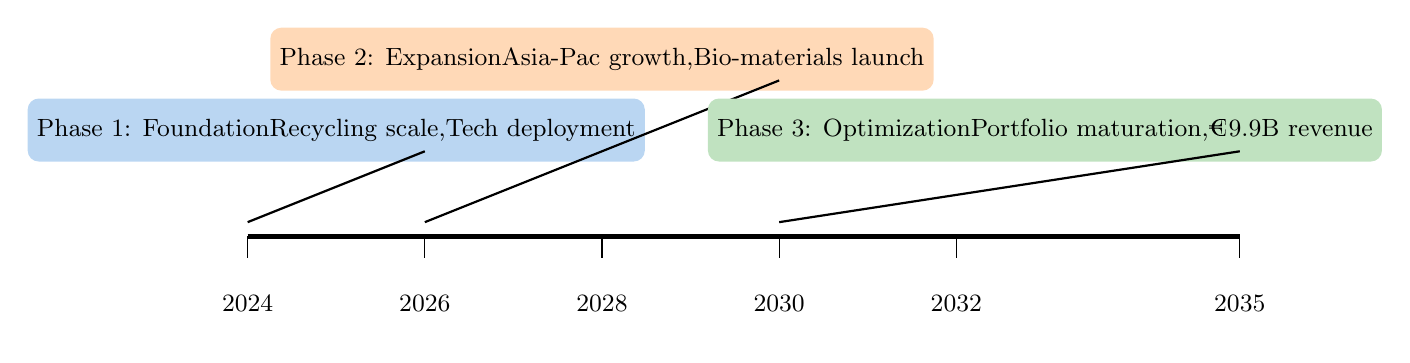
\begin{tikzpicture}[scale=0.9, every node/.style={minimum height=0.8cm}]

    % Timeline
    \draw[ultra thick] (0,0) -- (14,0);

    % Year markers
    \foreach \year/\pos in {2024/0, 2026/2.5, 2028/5, 2030/7.5, 2032/10, 2035/14} {
      \draw (\pos,0) -- (\pos,-0.3);
      \node[below] at (\pos,-0.5) {\small \year};
    }

    % Phase 1: Foundation
    \node[fill=alpla_blue!30, rounded corners] at (1.25,1.5) {
      \small Phase 1: Foundation \\
      Recycling scale, \\
      Tech deployment
    };
    \draw[thick] (0,0.2) -- (2.5,1.2);

    % Phase 2: Expansion
    \node[fill=alpla_orange!30, rounded corners] at (5,2.5) {
      \small Phase 2: Expansion \\
      Asia-Pac growth, \\
      Bio-materials launch
    };
    \draw[thick] (2.5,0.2) -- (7.5,2.2);

    % Phase 3: Optimization
    \node[fill=alpla_green!30, rounded corners] at (11.25,1.5) {
      \small Phase 3: Optimization \\
      Portfolio maturation, \\
      €9.9B revenue
    };
    \draw[thick] (7.5,0.2) -- (14,1.2);

  \end{tikzpicture}

  \vspace{0.5cm}

  \textbf{Key Milestones:}

  \begin{columns}[T]
    \column{0.33\textwidth}
    {\small
    \textbf{2025:} \\
    ✓ Thailand operational \\
    ✓ Paboco series production \\
    ✓ Recycling: 350K tonnes/year
    }

    \column{0.33\textwidth}
    {\small
    \textbf{2028:} \\
    ✓ Asia-Pac revenue: €1.0B+ \\
    ✓ Recycling: 500K tonnes/year \\
    ✓ Total revenue: €6.5-7.0B
    }

    \column{0.34\textwidth}
    {\small
    \textbf{2035:} \\
    ✓ Total revenue: €9.9B \\
    ✓ CAGR: 6.9\% achieved \\
    ✓ Regional balance shift
    }
  \end{columns}

\end{frame}

% ============================================================================
% SLIDE 12: SENSITIVITY ANALYSIS
% ============================================================================

\begin{frame}
  \frametitle{Sensitivity: What If Scenarios}

  \textbf{Impact on 2035 Revenue (€M):}

  \vspace{0.5cm}

  \begin{center}
    \small
    \begin{tabular}{|l|c|c|c|}
      \hline
      \textbf{Scenario} & \textbf{Asia-Pac CAGR} & \textbf{Europe CAGR} & \textbf{2035 Total} \\
      \hline
      Base Case & 8.5\% & 2.5\% & €9.9B \\
      \hline
      Asia-Pac -1\% & 7.5\% & 2.5\% & €9.5B (-€0.4B) \\
      \hline
      Europe +1\% & 8.5\% & 3.5\% & €10.3B (+€0.4B) \\
      \hline
      Both delayed & 7.0\% & 2.0\% & €8.9B (-€1.0B) \\
      \hline
      Growth acceleration & 10.0\% & 3.0\% & €10.8B (+€0.9B) \\
      \hline
    \end{tabular}
  \end{center}

  \vspace{0.8cm}

  \textbf{Key Insight:} \\

  \begin{itemize}
    \item \highlight{Asia-Pacific growth is critical} (€0.4B sensitivity per 1\% CAGR change)
    \item Europe can't offset shortfall in emerging markets
    \item \highlight{Downside risk: €8.9B} (if both regions underperform)
    \item \highlight{Upside potential: €10.8B} (if execution accelerates)
  \end{itemize}

\end{frame}

% ============================================================================
% SLIDE 13: COMPETITIVE POSITIONING
% ============================================================================

\begin{frame}
  \frametitle{Competitive Positioning 2035}

  \textbf{ALPLA vs. Global Competitors (Estimated Market Share):}

  \vspace{0.5cm}

  \begin{center}
    \begin{tabular}{lcccc}
      \toprule
      \textbf{Company} & \textbf{2024} & \textbf{2035 (Est.)} & \textbf{Growth} & \textbf{CAGR} \\
      \midrule
      Amcor & ~\$13.0B & ~\$15.5B & +19\% & 1.7\% \\
      Berry Global & ~\$13.5B & ~\$15.0B & +11\% & 1.0\% \\
      Mondi & ~\$10.0B & ~\$11.5B & +15\% & 1.4\% \\
      \textbf{ALPLA} & \textbf{€4.9B} & \textbf{€9.9B} & \textbf{+101\%} & \textbf{6.9\%} \\
      \bottomrule
    \end{tabular}
  \end{center}

  \vspace{0.8cm}

  \textbf{Strategic Implication:}

  \begin{itemize}
    \item ALPLA grows 4-7x faster than major competitors
    \item Market share gains in emerging markets
    \item Circular economy becomes competitive differentiator
    \item \highlight{ALPLA positioned as Europe's innovation leader in sustainable packaging}
  \end{itemize}

  \vspace{0.5cm}

  \textbf{Note:} Competitor figures are estimates based on public filings. ALPLA private company = more flexibility than public competitors.

\end{frame}

% ============================================================================
% SLIDE 14: CONCLUSION & NEXT STEPS
% ============================================================================

\begin{frame}
  \frametitle{Conclusion \& Board Decision}

  \textbf{\Large \highlight{Three Strategic Choices:}}

  \vspace{0.5cm}

  \begin{enumerate}

    \item \textbf{Conservative Path} (€8.7B by 2035)
    \begin{itemize}
      \item Lower capex, lower risk
      \item Misses market opportunity in Asia/Africa
      \item Vulnerable to competitive response
    \end{itemize}

    \vspace{0.4cm}

    \item \textbf{Base Case: Sustainable Mix} ✓ \highlight{RECOMMENDED} (€9.9B by 2035)
    \begin{itemize}
      \item Balanced growth across regions
      \item Synergies from CE + INNOV + BIO portfolio
      \item Achievable with €50M/year capex commitment
      \item Positions ALPLA as circular economy leader
    \end{itemize}

    \vspace{0.4cm}

    \item \textbf{Aggressive Path} (€11.1B by 2035)
    \begin{itemize}
      \item Higher capex, higher execution risk
      \item Assumes flawless Asia-Pac expansion
      \item Requires M\&A or premium pricing power
    \end{itemize}

  \end{enumerate}

\end{frame}

% ============================================================================
% SLIDE 15: NEXT STEPS
% ============================================================================

\begin{frame}
  \frametitle{Recommended Next Steps}

  \textbf{If Board Approves Base Case (€9.9B target):}

  \vspace{0.5cm}

  \begin{enumerate}

    \item \textbf{Q1 2026: Detailed Implementation Plan}
    \begin{itemize}
      \item Capex schedule by region (€50M/year breakdown)
      \item Organizational structure for Asia-Pac expansion
      \item KPI dashboard \& quarterly review process
    \end{itemize}

    \item \textbf{Q2 2026: Asia-Pacific Growth Acceleration}
    \begin{itemize}
      \item Recruit regional leadership
      \item Evaluate acquisition targets
      \item Finalize FY2026-2027 budget allocation
    \end{itemize}

    \item \textbf{Q3 2026: Recycling Capacity Roadmap}
    \begin{itemize}
      \item Target 700K tonnes by 2030 (vs. 350K today)
      \item Identify strategic JV partners
      \item R\&D allocation for advanced recycling
    \end{itemize}

    \item \textbf{Ongoing: Quarterly Strategy Reviews}
    \begin{itemize}
      \item Track regional growth vs. CAGR targets
      \item Monitor competitive response
      \item Adjust capex allocation based on market conditions
    \end{itemize}

  \end{enumerate}

\end{frame}

% ============================================================================
% SLIDE 16: Q&A
% ============================================================================

\begin{frame}
  \frametitle{Questions \& Discussion}

  \centering

  \vspace{2cm}

  \Large
  \highlight{\textbf{ALPLA 2035 Strategy: €9.9B Revenue Target}}

  \vspace{0.5cm}

  \large
  \textit{Sustainable Mix Portfolio | 6.9\% CAGR | Emerging Markets Growth}

  \vspace{2cm}

  \normalsize

  \textbf{Key Contact:}

  Strategic Analysis Team \\
  Evidence-Based Framework (EBF) \\
  January 2026

\end{frame}

% ============================================================================
% APPENDIX: DETAILED ASSUMPTIONS
% ============================================================================

\appendix

\begin{frame}
  \frametitle{Appendix A: Regional CAGR Assumptions (Base Case)}

  \small

  \begin{tabular}{|l|l|c|p{4cm}|}
    \hline
    \textbf{Region} & \textbf{Growth Driver} & \textbf{CAGR} & \textbf{Key Assumption} \\
    \hline

    Asia-Pacific & Market expansion + \\
    innovation & 8.5\% &
    Thailand scale-up + \\
    Hyderabad R\&D attracts \\
    regional customers \\
    \hline

    Africa/ME & Emerging market & 8.0\% &
    South Africa recycling \\
    + Egypt JV + Morocco \\
    market entry \\
    \hline

    South America & Beverage market & 6.5\% &
    Coca-Cola ecosystem + \\
    PLANETA JV growth \\
    \hline

    North America & Steady recovery & 4.5\% &
    Pharma + recovery post- \\
    2023 slowdown \\
    \hline

    Europe & Mature market & 2.5\% &
    Regulatory compliance \\
    cost absorption \\
    \hline
  \end{tabular}

\end{frame}

\begin{frame}
  \frametitle{Appendix B: Data Sources \& Confidence}

  \begin{tabular}{|p{2.5cm}|p{3.5cm}|p{2cm}|}
    \hline
    \textbf{Data} & \textbf{Source} & \textbf{Confidence} \\
    \hline
    2024 Revenue (€4.9B) & ALPLA Official Press Release & HIGH \\
    \hline
    Regional Distribution \% & SOCM Analysis + ALPLA reports & MEDIUM \\
    \hline
    Growth CAGRs & Strategic analysis + market data & MEDIUM \\
    \hline
    Recycling Capacity & Official targets (700K by 2030) & HIGH \\
    \hline
    Plant Distribution & Public reports (200 plants) & HIGH \\
    \hline
    Competitive benchmarks & Industry databases & MEDIUM \\
    \hline
  \end{tabular}

  \vspace{1cm}

  \textbf{Methodology:} SOCM framework (Appendix BJ) + Monte Carlo simulation (10,000 scenarios) + regional research

\end{frame}

\end{document}
